An overview of the system architecture, including the way in which the capabilities of new and emerging digital technologies have been leveraged, the types of data utilised and how the prototyped system supports the safe and secure routing of a diplomatic courier travelling from an initial location to a series of destinations in the world 

\section{Frontend}
\begin{itemize}
    \item Courier
    \item Supervisor
    \item Customer
\end{itemize}

\section{Backend}
\subsection{Customer database}
\begin{flushleft}
The first component of the backend is a database of customer and staff information. Its most important task is storing delivery information and constraints, which are merged with the maps database to provide directions to the courier. It is designed to store the following datatypes:
\end{flushleft}
\begin{minipage}{6.5cm}
    Customer: \{
    \begin{itemize} 
        \itemsep-0.5em
        \item[] customerId: id,
        \item[] name: string,
        \item[] address: string,
        \item[] postcode: string,
        \item[] city: string,
        \item[] country: string,
        \item[] publicKey: string,
        \item[] contactNumber: string,
        \item[] email: string,
        \item[] constraints: id
    \end{itemize}
    \}
\end{minipage}
\begin{minipage}{10cm}
    \hspace{1cm} \\
    \begin{itemize}
        \itemsep-0.5em
        \item[] \textit{unique customer identifier}
        \item[] \textit{customer name}
        \item[] \textit{address address}
        \item[] \textit{address postcode}
        \item[] \textit {address city}
        \item[] \textit{address country}
        \item[] \textit{customer public key, if known}
        \item[] \textit{customer phone number}
        \item[] \textit{customer email}
        \item[] \textit{identifier of customer constraint}
    \end{itemize}
    \hspace{1cm} \\
\end{minipage}
\begin{flushleft}
Every customer is a sender or receiver in a delivery: 
\end{flushleft}
\begin{minipage}{6.5cm}
    Delivery: \{
    \begin{itemize}
        \itemsep-0.5em
        \item[] deliveryId: id,
        \item[] sender: id,
        \item[] receiver: id,
        \item[] preferDestroy: boolean,
        \item[] customerMap: id,
        \item[] customerPublicKey: string,
        \item[] reinforcedBriefcase: boolean,
        \item[] lockMessage: string,
        \item[] couriers: [id],
        \item[] currentCourier: id,
        \item[]  supervisors: [id],
        \item[] constraints: id
    \end{itemize}
    \}
\end{minipage}
\begin{minipage}{10cm}
    \hspace{1cm} \\
    \begin{itemize}
        \itemsep-0.5em
        \item[] \textit{unique delivery identifier}
        \item[] \textit{sending customer id}
        \item[] \textit{receiving customer id}
        \item[] \textit{destroy package on capture preference}
        \item[] \textit{identifier of optional custom map}
        \item[] \textit{optional custom receiver public key}
        \item[] \textit{whether to use reinforced briefcase}
        \item[] \textit{reinforced briefcase password}
        \item[] \textit{identifiers of couriers handling the package}
        \item[] \textit{identifier of courier currently holding the package}
        \item[]  \textit{identifiers of supervisors handling the package}
        \item[] \textit{identifier of delivery constraint}
    \end{itemize}
    \hspace{1cm} \\
\end{minipage}
\begin{flushleft}
Every delivery links to a constraint object defining customer preferences.
\end{flushleft}
\begin{minipage}{7cm}
    Constraint: \{ 
    \begin{itemize}
        \itemsep-0.5em
        \item[] constraintId: id,
        \item[] active: boolean,
        \item[] bannedCountries: [string],
        \item[] bannedAirspaces: [string],
        \item[] bannedWaters: [string],
        \item[] bannedRoads: [string],
        \item[] allowedCar: boolean,
        \item[] allowedBoat: boolean,
        \item[] allowedFlight: boolean,
        \item[] allowedPublicTransport: boolean
        \item[] deadline: string
    \end{itemize}
    \}
\end{minipage}
\begin{minipage}{10cm}
    \hspace{1cm} \\
    \begin{itemize}
        \itemsep-0.5em
        \item[] \textit{unique identifier of constraint}
        \item[] \textit{whether constraint is in use}
        \item[] \textit{list of countries to avoid}
        \item[] \textit{list of airspaces to avoid}
        \item[] \textit{list of bodies of water to avoid}
        \item[] \textit{list of roads to avoid}
        \item[] \textit{(booleans specifying  which}
        \item[] \textit{methods of transport are allowed)}
        \item[] \hspace{1cm}
        \item[] \hspace{1cm}
        \item[] \textit{time by which delivery must occur (ISO format)}
    \end{itemize}
    \hspace{1cm} \\
\end{minipage}
\begin{flushleft}
Constraints exist on three levels: delivery, customer, and overall. Every delivery has its own constraints, allowing specific objects to be transported according to particular requirements. Every customer can have constraints applied to all of the deliveries where they are the sender. For example, government bodies may wish for none of their packages to cross countries they have strained diplomatic relations with. Finally, overall constraints are applied to all deliveries. These are applied when it becomes unsafe for anyone to traverse a particular area. Additional to these constraints we store staff contact and authentication data.
\end{flushleft}
\begin{minipage}{6.5cm}
    Courier: \{
    \begin{itemize}
        \itemsep-0.5em
        \item[] courierId: id,
        \item[] missionId: id,
        \item[] picture: string,
        \item[] name: string,
        \item[] publicKey: string,
        \item[] contactNumber: string,
        \item[] email: string,
        \item[] languages: [string],
        \item[] visas: [string],
        \item[] external: boolean,
        \item[] company: string
    \end{itemize}
    \}
\end{minipage}
\begin{minipage}{10cm}
    \hspace{1cm}
    \begin{itemize}
        \itemsep-0.5em
        \item[] \textit{unique identifier of courier}
        \item[] \textit{identifier of current delivery, if any}
        \item[] \textit{link to picture of courier}
        \item[] \textit{courier name}
        \item[] \textit{courier public key, for authentication}
        \item[] \textit{courier phone number}
        \item[] \textit{courier email}
        \item[] \textit{languages spoken by courier}
        \item[] \textit{visas courier possesses}
        \item[] \textit{whether the courier works for a different company}
        \item[] \textit{courier's company, if external}
    \end{itemize}
    \hspace{1cm}
\end{minipage}
\begin{flushleft}
The external and company attributes allow us to collaborate with other companies by outsourcing couriers.
\end{flushleft}
\begin{minipage}{6.5cm}
Supervisor: \{
\begin{itemize}
    \itemsep-0.5em
    \item[] supervisorId: id,
    \item[] name: string,
    \item[] contactNumber: string,
    \item[] email: string
\end{itemize}
\}
\end{minipage}
\begin{minipage}{10cm}
\hspace{1cm}
\begin{itemize}
    \itemsep-0.5em
    \item[] \textit{unique identifier of supervisor}
    \item[] \textit{supervisor's name}
    \item[] \textit{supervisor's phone number}
    \item[] \textit{supervisor's email address}
\end{itemize}
\hspace{1cm}
\end{minipage}
\begin{flushleft}
The database also stores all messages sent between staff on the private network.
\end{flushleft}
\begin{minipage}{6.5cm}
Message: \{
\begin{itemize}
    \itemsep-0.5em
    \item[] timestamp: string,
    \item[] message: string,
    \item[] fromType: string,
    \item[] fromId: string,
    \item[] toType: string,
    \item[] toId: string
\end{itemize}
\}
\end{minipage}
\begin{minipage}{10cm}
\hspace{1cm}
\begin{itemize}
    \itemsep-0.5em
    \item[] \textit{time the message was sent (ISO format)}
    \item[] \textit{message text}
    \item[] \textit{sender type (courier/supervisor)}
    \item[] \textit{sender's identifier}
    \item[] \textit{receiver type (courier/supervisor)}
    \item[] \textit{receiver's identifier}
\end{itemize}
\hspace{1cm}
\end{minipage}
\begin{flushleft}
Finally, the database stores an audit trail for every delivery, using objects called delivery events.
\end{flushleft}
\begin{minipage}{6.5cm}
DeliveryEvent: \{
\begin{itemize}
    \itemsep-0.5em
    \item[] deliveryId: id,
    \item[] timestamp: string,
    \item[] latitude: float,
    \item[] longitude: float,
    \item[] description: string,
    \item[] notes: string
\end{itemize}
\}
\end{minipage}
\begin{minipage}{10cm}
\hspace{1cm}
\begin{itemize}
    \itemsep-0.5em
    \item[] \textit{identifier of delivery}
    \item[] \textit{time at which event occurred (ISO format)}
    \item[] \textit{latitude at which event occurred}
    \item[] \textit{longitude at which event occurred}
    \item[] \textit{description of event (e.g. "delivered")}
    \item[] \textit{optional additional notes}
\end{itemize}
\hspace{1cm}
\end{minipage}
\begin{figure}[h]
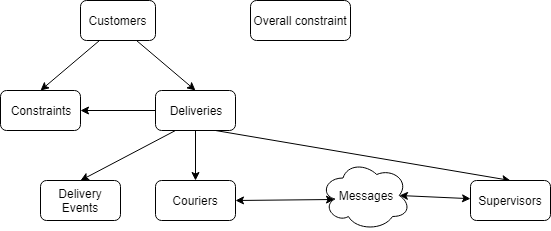
\includegraphics[scale=0.5]{database_outline.png}
    \centering
    \caption{Outline of Redis database}
    \label{fig:redis_database}
\end{figure}
\begin{flushleft}
This information will be stored in a Redis database within a Docker image, for ease of setup and added security. Redis was chosen for its efficiency and security-- it is a simple database designed with speed in mind, and has measures in place to avoid third party attacks\cite{redisSecutiry}. It allows us to rename and disable commands such that potential attackers cannot send commands to the database. We will use this to ban clearing the database contents, and obscure all commands used by the API code. Redis has no concept of string escaping, making injection attacks impossible. It does not support encryption, but to compensate for this we will use a firewall to block all but the API server from communicating with it, and encrypt all API responses.
\end{flushleft}
\begin{flushleft}
A set of Python functions will be defined to verify and process data sent to Redis such that it contains the attributes and data types described. These functions are to be used by a class called RedisInterface. This is a wrapper around the Redis Python package, implementing functions for adding and retrieving all of the above objects.
\end{flushleft}
\begin{flushleft}
An API layer will be written on top of this using Flask, allowing the frontend to access, update, and delete data without needing knowledge of which RedisInterface methods to call. This API will also be enclosed in a Docker image, allowing us full control of the API server. The architecture of the Redis API is summarised in the following figure.
\end{flushleft}
\begin{figure}[h]
    \centering
    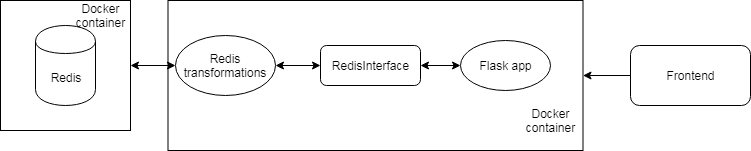
\includegraphics[scale=0.5]{redis_backend_diagram.png}
    \caption{Redis API software architecture}
    \label{fig:redis_architecturel}
\end{figure}
\begin{flushleft}
The API is designed with the database structure in mind, providing simple links to constraints on all levels, lists of staff and customers, as well as specific information retrievable by ID. The following table provides a list of URLs, callable methods, and expected API responses.
\end{flushleft}
\begin{center}
\begin{tabular}{ | m{6.1cm} | m{3.8cm}| m{6cm} | } 
\hline
URL & Methods & Description \\
\hline
/constraints/overall & GET, POST, DELETE & Get, modify, or remove overall constraints \\
\hline
/constraints/customer/<customerId> & GET, POST, DELETE & Get, modify, or remove a specific customer's constraints \\
\hline
/constraints/delivery/<deliveryId> & GET, POST, DELETE & Get, modify, or remove a specific delivery's constraints\\
\hline
/customers & GET, POST & Get the full list of customers, or add a customer\\
\hline
/customers/<customerId> & GET, PUT, DELETE & Get, update, or remove a customer's data\\
\hline
/couriers & GET, POST & Get the full list of couriers, or add a courier\\
\hline
/couriers/<courierId> & GET, PUT, DELETE & Get, update, or remove a courier's data\\
\hline
/supervisors & GET, POST & Get the full list of supervisors, or add a supervisor\\
\hline
/supervisors/<supervisorId> & GET, PUT, DELETE & Get, update, or remove a supervisor's data\\
\hline
/deliveries & GET, POST & Get the full list of deliveries, or add a delivery\\
\hline
/deliveries/<deliveryId> & GET, PUT, DELETE & Get, update, or remove a delivery\\
\hline
/deliveries/customer/<customerId> & GET & Get all deliveries where a particular customer is either sender or receiver\\
\hline
/events/<deliveryId> & GET & Get all of a delivery's events\\
\hline
/messages & GET, POST & Get all messages sent or received by a specific person, or add a message\\
\hline
\end{tabular}
\end{center}
\subsection{Maps API}
\section{Communication}

\section{Briefcase}
The design of the briefcase must be considered from both a hardware and software perspective. The general design of the hardware system is shown in Fig. \ref{fig:briefcase_architecture}. All peripherals in the system are represented as circles in Fig. \ref{fig:briefcase_architecture}, while intermediate components are represented as rectangles.
\begin{figure}[h]
    \centering
    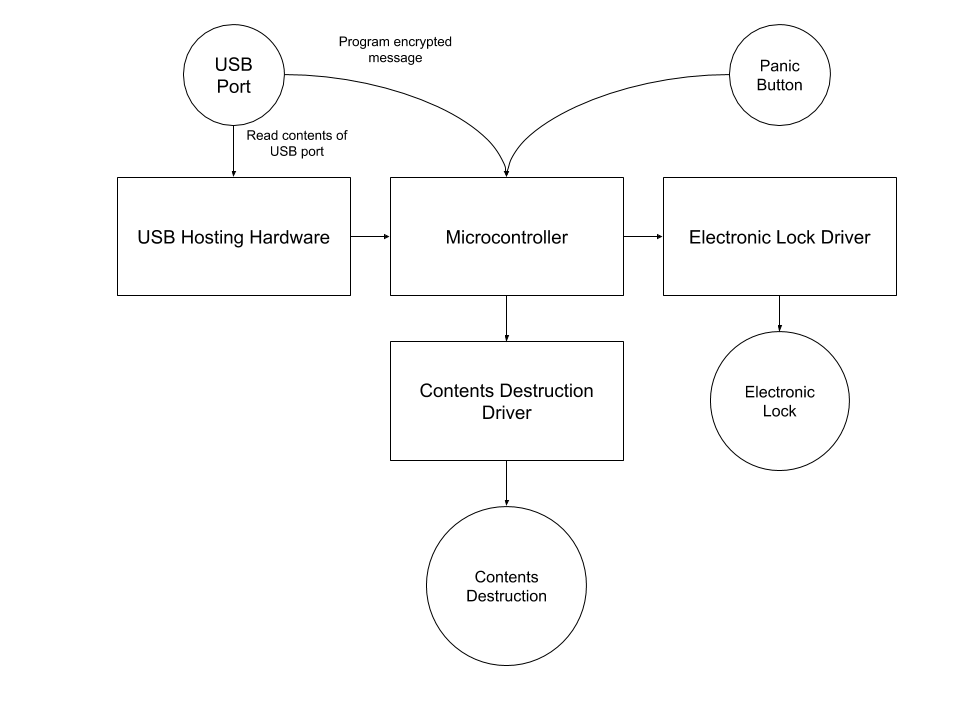
\includegraphics[scale=0.4]{Briefcase_Architecture_Diagram.png}
    \caption{Briefcase Hardware Architecture}
    \label{fig:briefcase_architecture}
\end{figure}

As it is common for microcontrollers to not have USB hosting capabilities, USB hosting hardware is required to read the contents of a memory stick that is plugged into the concealed USB port. This hardware could be similar to the hardware found on the Arduino USB Host Shield \cite{arduinoUSBHost}, or a microcontroller with USB On-The-Go (OTG) capabilities \cite{techopediaUSBOTG} such as the 